%%%%%%%%%%%%%%%%%%%%%%%%%%%%%%%%%%%%%%%%%%%%%%%%%%%%%%%%%%%%%%%%%%%%
%% %%	Posterdown PDF class for LaTeX files	 08-JAN-2019
%% %%	For any information please send an e-mail to:
%% %%		brentthonre18@gmail.com (Brent Thorne)
%% %%
%% %%	Initial class provided by:
%% %%		Brent Thorne
%%%%%%%%%%%%%%%%%%%%%%%%%%%%%%%%%%%%%%%%%%%%%%%%%%%%%%%%%%%%%%%%%%%%

%% THIS HAS BEEN MODIFIED BY SHEA CONNELL TO CONFORM WITH THE NEEDS
%% FOR THE EACR TRACKING CANCER CONFERENCE

\documentclass[article,30pt,extrafontsizes]{memoir}



%utf-8 seems to be important
\RequirePackage[utf8]{inputenc}
\RequirePackage[T1]{fontenc}
\RequirePackage{lmodern}
\RequirePackage{multicol}
\RequirePackage{graphicx}
\RequirePackage{blindtext}
\RequirePackage[svgnames,table]{xcolor}
\RequirePackage{tikz}
\RequirePackage[framemethod=tikz]{mdframed}
\RequirePackage{color}
\RequirePackage{geometry}
\RequirePackage{adjmulticol}
\RequirePackage{epstopdf}
\RequirePackage{stfloats}
\RequirePackage[export]{adjustbox}
\RequirePackage[norule,symbol]{footmisc}
\RequirePackage{placeins}
\RequirePackage[none]{hyphenat}
\RequirePackage[font=small,labelfont=bf]{caption}
%For kable extra package :)
\RequirePackage{booktabs}
\RequirePackage{longtable}
\RequirePackage{array}
\RequirePackage{multirow}
\RequirePackage{wrapfig}
\RequirePackage{float}
\RequirePackage{colortbl}
\RequirePackage{pdflscape}
\RequirePackage{pagecolor}
\RequirePackage{tabu}
\RequirePackage{threeparttable}
\RequirePackage{threeparttablex}
\RequirePackage[normalem]{ulem}
\RequirePackage{makecell}
\RequirePackage{wrapfig}

%%%%%%%%% COLOURS %%%%%%%%

%Fill/ Line Colours
\definecolor{titlebgcol}{HTML}{690F8C}
\definecolor{columnlinecol}{HTML}{000000}
\definecolor{posterbgcol}{HTML}{ffffff}
\definecolor{headerbgcol}{HTML}{008080}

% Text Colours
\definecolor{titletextcol}{HTML}{ffffff}
\definecolor{authortextcol}{HTML}{E5E5E5}
\definecolor{affiliationtextcol}{HTML}{B6B6B6}
\definecolor{headertextcol}{HTML}{690F8C}
\definecolor{bodytextcol}{HTML}{000000}
\definecolor{footnotetextcol}{HTML}{000000}
\definecolor{citecol}{HTML}{CC0000}
\definecolor{urlcol}{HTML}{008080}
\definecolor{linkcol}{HTML}{ffffff}

\RequirePackage{hyperref}
\hypersetup{
    colorlinks=true,
    linkcolor=linkcol,
    citecolor=citecol,
    filecolor=magenta,
    urlcolor=urlcol,
}

%For figure and table placement
\RequirePackage{float}
\floatplacement{figure}{H}
\floatplacement{table}{H}

%spacing between figure/ table and caption
\setlength{\abovecaptionskip}{0.4in}
\setlength{\belowcaptionskip}{0.2in}
\captionnamefont{\footnotesize\sffamily\bfseries}
\captiontitlefont{\footnotesize\sffamily}

%define column options
\setlength{\columnseprule}{1pt}
\def\columnseprulecolor{\color{columnlinecol}}

\setsubsubsecheadstyle{\small\color{headertextcol}\textbf}% Set \section style
\setsecheadstyle{\small\color{headertextcol}}
\setsecnumformat{}
\def\sectionmark#1{\markboth{#1}{#1}}

%-----------------------------------------------------

\thispagestyle{empty}
\definecolor{light-gray}{gray}{0.9}

%biblatex options
\RequirePackage[sorting=none,backend=biber,style=numeric-comp]{biblatex}
\renewcommand*{\bibfont}{\tiny}
\bibliography{MyLibrary}
\defbibheading{bibliography}[\bibname]{%
\setlength\bibitemsep{0.4\itemsep}
\section*{#1}%
\markboth{#1}{#1}}
\AtBeginDocument{%
  \renewcommand{\bibname}{References}
}

%bring in the users information
\author{\large\textbf{Shea P. Connell}\normalsize\textsuperscript{1}, Marcel
Hanna\textsuperscript{1}, Frank McCarthy\textsuperscript{2}, Rachel
Hurst\textsuperscript{1}, Helen Curley\textsuperscript{1}, Martyn
Webb\textsuperscript{1}, Helen Walker\textsuperscript{3}, Rob
Mills\textsuperscript{3}, Richard Y. Ball\textsuperscript{3}, Martin G.
Sanda\textsuperscript{4}, Kathryn L. Pellegrini\textsuperscript{4},
Dattatraya Patil\textsuperscript{4}, Antoinette S.
Perry\textsuperscript{5}, Jack Schalken\textsuperscript{6}, Hardev
Pandha\textsuperscript{7}, Hayley Whitaker\textsuperscript{8}, Nening
Dennis\textsuperscript{2}, Christine Stuttle\textsuperscript{2}, Ian G.
Mills\textsuperscript{9,10,11}, Ingrid Guldvik\textsuperscript{10}, The
Movember GAP1 Urine Biomarker Consortium, Chris
Parker\textsuperscript{2,12}, Jeremy Clark\textsuperscript{1}, Daniel S.
Brewer\textsuperscript{1,13}, Colin S. Cooper\textsuperscript{1}}
\title{\fontfamily{phv}\selectfont Predicting outcome in prostate cancer
patients using a multi-signature risk classifier, derived from urinary
extracellular vesicles}
\counterwithout{section}{chapter}
\makechapterstyle{mydefault}{
\addtocounter{secnumdepth}{2}
\setsecheadstyle{\centering\Large\color{headertextcol}\textbf}
\setsubsecheadstyle{\itshape}
\setsubsubsecheadstyle{\itshape}
}

\chapterstyle{mydefault}

%define column spacing
\setlength\columnsep{1in}

\setlength\parindent{1em}
\setlength\parskip{1em}
\setlength\hangparas{0}

%spacing after section head title
\setaftersecskip{0.3in}
\setbeforesecskip{1in}
\setlength\textfloatsep{0.3in}
\setlength\floatsep{0.3in}
\setlength\intextsep{0.3in}

\setstocksize{140cm}{90cm}
\settrimmedsize{\stockheight}{\stockwidth}{*}
\settypeblocksize{140cm}{90cm}{*}
\setlrmargins{*}{*}{1}
\setulmarginsandblock{2.5cm}{0cm}{*}
\setmarginnotes{0em}{0cm}{0cm}
\setlength{\footskip}{0cm}
\setlength{\footnotesep}{0cm}
\setlength{\headheight}{0pt}
\setlength{\headsep}{0pt}
\setlength{\trimtop}{0pt}
\setlength{\trimedge}{0pt}
\setlength{\uppermargin}{0pt}
\checkandfixthelayout


\mdfdefinestyle{brentsmdfstyle}{%
  backgroundcolor=titlebgcol,
  linecolor=columnlinecol,
  topline=false,
  leftline=false,
  rightline=false,
  linewidth=2mm}

%Footnote to white
\RequirePackage{footmisc}
\def\footnotelayout{\centering\color{footnotetextcol}}

%Allows for the use of blank, un-numbered footnotes
\newcommand\blfootnote[1]{%
  \begingroup
  \renewcommand\thefootnote{}\footnote{#1}%
  \addtocounter{footnote}{-1}%
  \endgroup
}

% see https://stackoverflow.com/a/47122900

% choose font family
\RequirePackage{palatino}

\newpagecolor{posterbgcol}

%begin the document
\begin{document}
\begin{mdframed}[style=brentsmdfstyle]

%sets footnote to be white hopefully
\renewcommand*\footnoterule{}
\renewcommand{\thempfootnote}{\footnotesize\color{footnotetextcol}{\arabic{mpfootnote}}}

% group which adds title author and other infor
% Used instead of \maketitle for better spacing options
\begingroup
  \centering
  \color{titletextcol}
\vspace{0.5in}
  \Huge{\fontfamily{phv}\selectfont Predicting outcome in prostate cancer
patients using a multi-signature risk classifier, derived from urinary
extracellular vesicles}  \\[0.3in]
  \color{authortextcol} \normalsize{\large\textbf{Shea P. Connell}\normalsize\textsuperscript{1}, Marcel
Hanna\textsuperscript{1}, Frank McCarthy\textsuperscript{2}, Rachel
Hurst\textsuperscript{1}, Helen Curley\textsuperscript{1}, Martyn
Webb\textsuperscript{1}, Helen Walker\textsuperscript{3}, Rob
Mills\textsuperscript{3}, Richard Y. Ball\textsuperscript{3}, Martin G.
Sanda\textsuperscript{4}, Kathryn L. Pellegrini\textsuperscript{4},
Dattatraya Patil\textsuperscript{4}, Antoinette S.
Perry\textsuperscript{5}, Jack Schalken\textsuperscript{6}, Hardev
Pandha\textsuperscript{7}, Hayley Whitaker\textsuperscript{8}, Nening
Dennis\textsuperscript{2}, Christine Stuttle\textsuperscript{2}, Ian G.
Mills\textsuperscript{9,10,11}, Ingrid Guldvik\textsuperscript{10}, The
Movember GAP1 Urine Biomarker Consortium, Chris
Parker\textsuperscript{2,12}, Jeremy Clark\textsuperscript{1}, Daniel S.
Brewer\textsuperscript{1,13}, Colin S. Cooper\textsuperscript{1}} \\[0.2in]
  \color{affiliationtextcol} \footnotesize{\textsuperscript{1} Norwich Medical School, University of East Anglia,
UK; \textsuperscript{2} The Institute of Cancer Research, UK;
\textsuperscript{3} Norfolk and Norwich University Hospitals NHS
Foundation Trust, UK; \textsuperscript{4} Department of Urology, Winship
Cancer Institute, Emory University School of Medicine, USA;
\textsuperscript{5} Cancer Biology and Therapeutics Laboratory, School
of Biology and Environmental Science, Conway Institute, University
College Dublin, Ireland; \textsuperscript{6} Nijmegen Medical Centre,
Radboud University Medical Centre, The Netherlands; \textsuperscript{7}
Faculty of Health and Medical Sciences, The University of Surrey, UK;
\textsuperscript{8} Molecular Diagnostics and Therapeutics Group,
University College London, UK; \textsuperscript{9} School of Medicine,
Dentistry and Biomedical Sciences, Institute for Health Sciences, Centre
for Cancer Research and Cell Biology, Queen's University Belfast, UK;
\textsuperscript{10} Centre for Molecular Medicine, University of Oslo,
Norway; \textsuperscript{11} Nuffield Department of Surgical Sciences,
University of Oxford, UK; \textsuperscript{12} The Royal Marsden
Hospital, Sutton, UK; \textsuperscript{13} The Earlham Institute,
Norwich Research Park, UK}
  \vspace{0.2in}

% end title section -------------------
  \endgroup
\end{mdframed}

%include the 4-Risk plots:
\graphicspath{ {Figures/} }
\begin{figure}
  \centering
  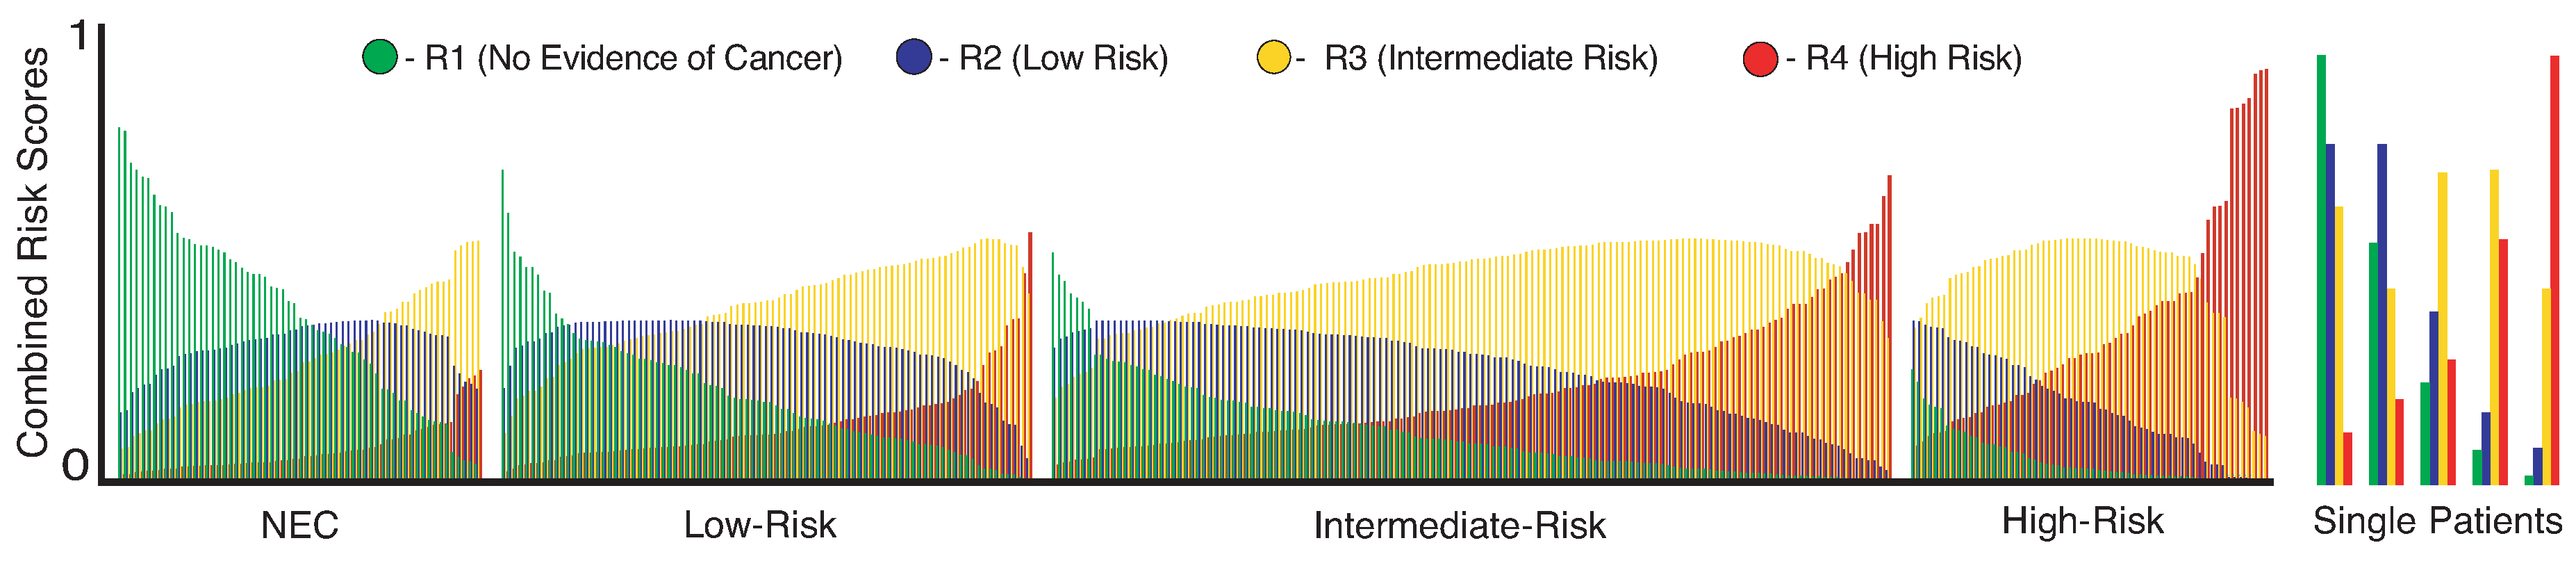
\includegraphics[width=0.96\linewidth]{RiskProfiles}
  \vspace{-10mm}
  \captionsetup{width=.95\linewidth}
  \caption{Combined risk profiles of the entire Movember cohort, grouped by D’Amico risk category and ordered by ascending R4 score.
  Each individual patient has four signatures associated with their sample, detailing the membership probability of their sample to normal tissue (R1 - green), D’Amico Low-risk (R2 - blue), Intermediate-risk (R3 - yellow), and High-risk (R4 - red). Example profiles of individual patients are shown on the right.}
\end{figure}
% Begin body of poster
\begin{adjmulticols*}{2}{10mm}{10mm}
\normalsize{
\color{bodytextcol}
\begin{figure}
\definecolor{bordercolour}{HTML}{DCDCDC}
\definecolor{titleColour}{HTML}{252525}
\definecolor{myframecolour}{HTML}{690F8C}
\mdfsetup{frametitlealignment=\center,
          frametitlefont=\fontfamily{ppl}\selectfont,
          frametitlefont=\huge,
          frametitlebackgroundcolor=bordercolour,
          frametitlefontcolor = titleColour,
          linecolor=black,
          linewidth=5pt}
\begin{mdframed}[backgroundcolor = myframecolour,
                  font = \fontfamily{ppl}\selectfont,
                  fontcolor = white, 
                  roundcorner = 20pt, 
                  innerleftmargin = 30pt,
                  innerrightmargin = 30pt,
                  frametitle={\textbf{Quick Read}}]

\Large\textbf{Question: }\large Can a non-invasive single-sample urine test reveal \textbf{both diagnostic \& prognostic information about 537 prostate cancer patients}, utilising extracellular vesicle-derived RNA expression patterns?\bigskip\\
\Large\textbf{Findings: }\large A robust, four-risk-signature model identified two groups with differing rates of treatment intervention in active surveillance use (\textbf{High Risk HR = 3.7, Low Risk HR = -7.0}) \& predicted initial biopsy outcome (\textbf{AUC = 0.81})\bigskip\\
\Large\textbf{Impact: }\large Clinical implementation of this model has the potential to \textbf{avoid the unnecessary initial biopsy of men} \& the repeated, invasive follow-up of men on active surveillance with indolent prostate cancer could be drastically reduced, or \textbf{provide a means for exiting surveillance altogether}. 
\end{mdframed}
\end{figure}
\vspace{-45mm}

\hypertarget{introduction}{%
\section{Introduction}\label{introduction}}

\vspace{-7.5mm}

\textbf{Clinical problem:} To combat the over-treatment of men with
indolent prostate cancer, men with D'Amico Low \& favourable
Intermediate risk cancers are often offered active surveillance (AS) as
an option\textsuperscript{\cite{Selvadurai2013}}. Involving regular
assessment for signs of disease progression, AS has proven successful in
reducing unnecessary treatment.But invasive and repeated assessment
means elective treatment rates can be higher than
30\%\textsuperscript{\cite{Hamdy2016}} and there is no formal method for
patients to exit AS.

\textbf{Rationale:} Previous studies established urine as a suitable
medium for non-invasive sampling of the
prostate\textsuperscript{\cite{McKiernan2016b,Tomlins2016a,Donovan2015,VanNeste2016}}.
In this vein, we have developed a risk prediction model, using
NanoString quantified RNA expression from urinary extracellular
vesicles, with the aim to discriminate accurately between men with, and
without, clinically significant cancers. \vspace{-28.5mm}

\hypertarget{the-movember-cohort}{%
\section{The Movember Cohort}\label{the-movember-cohort}}

\vspace{-7.5mm}

\textbf{Patients \& Samples:} Post-DRE urine from 537 men with and
without histologically proven cancer with a PSA \textless{} 100 ng/mL,
collected from urology clinics in the UK, Ireland and USA between 2009
and 2015. Extracellular vesicle RNA profiles derived with NanoString.
Biopsy information from trans-rectal ultrasound guided needle biopsy.

\textbf{AS Eligibility \& Progression:} Age 50--80, clinical stage
T1/T2, PSA \textless{} 15 ng/mL, Gs \textless{}7 (Gs \textless{} 4+3 if
age \textgreater{}65), and \textless{}50\% percent positive biopsy
cores. Progression was defined as PSA velocity \textgreater{}1 ng/mL per
year or adverse histology on repeat biopsy, defined as primary G
\textgreater{}3 or \textgreater{}50\% biopsy cores positive for cancer.

\vspace{-28.5mm}

\hypertarget{methods}{%
\section{Methods}\label{methods}}

\vspace{-7.5mm}

\textbf{Model:} Continuation-ratio LASSO regression trained on 67\% of
the data \& treating D'Amico risk status as an ordinal variable. Four
risk signatures generated predicted probabilities of normal tissue (R1),
D'Amico Low-risk (R2), Intermediate-risk (R3), and High-risk (R4) PCa in
a given sample.

\textbf{Testing:} ROC-AUC analysis tested prediction of biopsy outcome
in the remaining 33\% test dataset. Survival analyses assessed
prognostication of disease progression of patient in an AS sub-cohort
with long follow-up(n = 87, \textgreater{}5 years). \vspace{-28.5mm}

\hypertarget{results}{%
\section{Results}\label{results}}

\vspace{-7.5mm}

\textbf{Prediction of D'Amico Risk \& biopsy outcome}: There was a
strong association with clinical category, appearing to recategorise
approximately 15\% of samples at either end of each D'Amico risk group
(Figure 1). AUC of a clinically significant initial biopsy outcome of
D'Amico Intermediate- or High-Risk: \textbf{0.813 (95\% CI: 0.779 -
0.847, Figure 2)}.

\textbf{AS Prognostication} Two groups, dichotomised by a robust R4
threshold had large differences in time to progression; 60\% of those
deemed high risk progressed whilst only 10\% of low risk patients
progressed 5 years from urine sample collection: (Figure 3, median
progression 26\%). Cox models detailed significant differences in
progression; \textbf{R4 HR = 3.71 (95\% CI: 1.53 to 5.89)}, and
\textbf{R1 HR =-7.03 (95\% CI: -12.29 to -1.77)}. \vspace{-28.5mm}

\hypertarget{conclusion}{%
\section{Conclusion}\label{conclusion}}

\vspace{-7.5mm}

Clinical implementation of our model for biopsy prediction could reduce
the rate of unnecessary initial biopsy, performing similarly to
previously published urine tests for clinically significant cancers.
However, no other test currently exists to prognosticate AS patients as
we have shown. The model has the potential identify men at particular
risk of progression, or, more importantly, those who may be safely left
alone for up to five years.\\

\begin{figure}

{\centering \includegraphics[width=1\linewidth,trim={0 5mm 0 10mm},clip]{Poster_files/figure-latex/unnamed-chunk-2-1} 

}

\caption{ROC-AUC plot of the ability of R4 to predict the presence of D'Amico Intermediate or High risk cancer on initial biopsy. Shaded region indicates 95\% confidence intervals from 2000 bootstrap resamples.}\label{fig:unnamed-chunk-2}
\end{figure}
\vspace{-10mm}

\begin{figure}

{\centering \includegraphics[width=1\linewidth,trim={0 2.5mm 0 2.5mm},clip]{Poster_files/figure-latex/unnamed-chunk-3-1} 

}

\caption{Kaplan-Meier plot of time to disease progression in months from initial urine collection. Colours indicate the dichotomised model thresholds, Green – Low R4, Red – High R4. Numbers above the x-axis indicate the number of patients in each group at risk at the given time intervals. Shaded regions indicate 95\% confidence intervals.}\label{fig:unnamed-chunk-3}
\end{figure}

\vspace{-15mm}
\begin{figure}
\printbibliography 
\vspace{0mm}
\centering

\includegraphics[clip=true,width = 38cm]{Affiliations}
\end{figure}
\vspace{-60mm}

\blfootnote{\newline All analyses presented were undertaken in R, with the poster produced through the `posterdown` package. All of the code \& data needed to reproduce this poster exactly as seen can be found at \textbf{https://github.com/Shedimus/EACR-Tracking-Cancer}\raisebox{-.4\height}{
\includegraphics[clip=true,width = 4cm]{GitHubQR}}}
}
\end{adjmulticols*}
%end the poster
\end{document}
